\documentclass{article}

\usepackage[utf8]{inputenc}
\usepackage[T1]{fontenc}
\usepackage{lipsum}
\usepackage{graphicx}
\usepackage{amsmath}
\usepackage[margin=1in]{geometry}
\usepackage{titlesec}
\usepackage{graphicx}
\usepackage{floatflt,epsfig}
\usepackage[utf8]{inputenc}
\usepackage[T1]{fontenc}
\usepackage{lipsum}
\usepackage{graphicx}
\usepackage{amsmath}
\usepackage[margin=1in]{geometry} 
\usepackage{titlesec}
\usepackage{listings}
\usepackage{xcolor}

\lstdefinelanguage{XML}
{
  morestring=[b]",
  morestring=[s]{>}{<},
  morecomment=[s]{<?}{?>},
  morecomment=[s][\color{green!50!black}]{<!--}{-->},
  stringstyle=\color{blue},
  identifierstyle=\color{red},
  keywordstyle=\color{orange},
  commentstyle=\color{green!50!black},
  basicstyle=\small\ttfamily,
  frame=single, 
  breaklines=true,
  breakatwhitespace=true,
  tabsize=2,
  showstringspaces=false,
  captionpos=b,
}

\lstdefinelanguage{Java}{
  keywords={abstract,assert,boolean,break,byte,case,catch,char,class,const,continue,default,do,double,else,enum,extends,false,final,finally,float,for,goto,if,implements,import,instanceof,int,interface,long,native,new,null,package,private,protected,public,return,short,static,strictfp,super,switch,synchronized,this,throw,throws,transient,true,try,void,volatile,while},
  morekeywords={[2]System,out},
  morecomment=[l]{//},
  morecomment=[s]{/*}{*/},
  morestring=[b]",
  basicstyle=\small\ttfamily,
  keywordstyle=\color{blue}\bfseries,
  keywordstyle={[2]\color{orange}\bfseries},
  commentstyle=\color{green!70!black},
  stringstyle=\color{red},
  showstringspaces=false,
  tabsize=2,
  breaklines=true,
  breakatwhitespace=true,
  frame=single, 
  captionpos=b
}


\titleformat{\section}
{\LARGE\bfseries}{\thesection}{1em}{}

\titleformat{\subsection}
{\Large\bfseries}{\thesection}{1em}{}

\begin{document}

\pagestyle{empty}

\section*{Views}
\large
\textbf{Android Views} è il paradigma standard per la creazione e manipolazione di tutti gli elementi grafici che compongano la \textit{User Interface}. Una \textbf{View} definisce un concetto primitivo ma essenziale per lo sviluppo di applicazioni, contenitrice di tutti gli oggetti visualizzati a schermo. Pertanto una \textit{View} è responsabile non solo della modellazione di tutti gli elementi grafici che caratterizzano l'applicazione di riferimento, ma anche della gestione degli eventi che li riguardano, come l'interazione con agenti esterni oppure l'acquisizione di dati.\vspace*{14pt}\\
Esempi più comuni di \textit{View} sono distinti in:
\begin{enumerate}
  \itemsep0em
  \renewcommand{\labelenumi}{-}
  \item \textbf{Widgets}, descritte come delle etichette, da non confondere con il sistema software già in uso all'interno di dispositivi mobili
  \item \textbf{Layouts}, insieme di caratteristiche grafiche e comportamentali    
\end{enumerate} 
Per determinare una \textit{View} si adottano due metodi essenziali:
\begin{enumerate}
  \itemsep0em
  \renewcommand{\labelenumi}{-}
  \item \textbf{Declarative method}, metodo dichiarativo di una \textit{View} tramite il file \textit{XML}, simile a quanto definito a livello di \textit{Activity}, in cui il \textit{Manifest} assume un'importanza essenziale. Il loro accesso tramite linguaggi di programmazione, \textit{Java} oppure \textit{Kotlin}, avviene tramite il metodo \textbf{findViewById()} a cui è passato come parametro l'elemento grafico contenuto all'interno della medesima \textit{View}\\
  \begin{lstlisting}[language=XML]
<TextView
  android:id = "@+id/myTextView"
  android:layout_width = "match_parent"
  android:layout_height = "wrap_content"
  android:text = "Hello World"
  android:textAlignment = "center"
  title=Dichiarazione all'interno del file XML
/>
  \end{lstlisting}
  \begin{lstlisting}[language=JAVA, title=Dichiarazione all'interno del file XML]
    public TextView textView;
    textView = (TextView)findViewById(R.id.myTextView);
  \end{lstlisting}
  \item \textbf{Programmatic View}, in questo ambito le \textit{View} sono direttamente create in \textit{Java} o \textit{Kotlin}, immettendo il \textit{contesto} di riferimento. Tuttavia si tratta di un approccio non raccomandato, a causa del fatto che nella sezione \textit{code} occorre dettare tutte le proprietà visive        
\end{enumerate} 

\subsection*{Handling Events}
La fase successiva ritrae la gestione degli eventi associati agli oggetti visivi. \textit{Java}/\textit{Kotlin} manipolano i possibili eventi attraverso la keyword \textbf{OnClick}; mediante la stessa definizione è possibile addirittura forzare l'avvenimento di un evento senza alcuna interazione.\vspace*{14pt}\\
Esistono tre differenti metodi per gestire gli eventi, suddivisi in:
\begin{enumerate}
  \itemsep0em
  \renewcommand{\labelenumi}{-}
  \item \textbf{XML}, il tutto gestito mediante le \textbf{callbacks}, direttamente indicate nel file; tuttavia il metodo descritto riguarda solamente un numero ristretto di componenti. \\METTERE ESEMPIO SLIDE 10
  \item \textbf{Event Handlers}, in questa sezione ogni \textit{View} contiene un ammontare di metodi, richiamati qualora dovesse verificarsi un evento. Le differenti funzioni citate sono frutto di innumerevoli \textit{extend} adattati nella classe \textit{View}, riferiti agli oggetti grafici, per cui tramite questo approccio occorre compiere molteplici \textit{override}; di conseguenza più articolata risulterà la \textit{View}, maggiore sarà l'\textit{impraticabilità}
  \item \textbf{Event Listeners}, in quest'ultima casistica, ogni \textit{View} delega l'implementazione del comportamento, successivo ad un certo evento, ad un oggetto. In tal senso, ogni \textit{listener} gestisce una singola tipologia di evento e contiene un unico metodo \textit{callback}. Si evince in questa breve descrizione la volontà di dividere nettamente ciò che è ritenuto dinamico, come l'interfaccia grafica, da elementi che costituiscono la logica dell'applicazione, ossia il comportamento successivo alla veridicità dell'evento, sovrapponendo un layer di astrazione in grado di isolare le due entità da modifiche e cambiamenti reciproci. \\
  \begin{lstlisting}[language=JAVA, title=Gestione evento tramite Event Listener]
Button button;
class MainActivity extends AppCompatActivity implements OnClickListener{
  @Override
  protected void onCreate(Bundle savedInstanceState) {
    ...
    button = findViewById(R.id.button1);
    button.setOnClickListener(this); 
  }

  @Override 
  void onClick(View v) { }
}
  \end{lstlisting}
  Di seguito sono definiti brevemente gli aspetti salienti della sezione di codice riportata:
  \begin{itemize}
    \itemsep0em
    \item In questo esempio la \textit{MainActivity} implementa la classe astratta \textit{OnClickListener}, affinchè possa gestire correttamente gli eventi scaturiti da interazioni con agenti esterni
    \item All'interno del metodo \textit{onCreate()}, viene acquisito il bottone immesso all'interno della \textit{View}. In questo modo è possibile, attraverso il \textit{listener}, definire il comportamento del bottone una volta creato; si ricorda che la gestione e il coordinamento degli eventi avviene tramite la keyword \textit{OnClick}
    \item Infine all'interno del metodo \textit{onClick()}, da cui si osserva la keyword \textit{Override}, è sviluppata la vera logica del bottone, rispettando in questo modo la suddivisione in business logic e classi di alto livello descritta precedentemente. Nel caso in cui dovessero essere presenti più bottoni occorrerà implementare uno \textit{switch} che possa distinguere le possibili casistiche
  \end{itemize}
\end{enumerate}

\subsection*{Layout}
Un \textbf{Layout} deve estendere una \textbf{ViewGroup}. Una \textit{ViewGroup} è un contenitore di \textit{View} adottato per definire la struttura del loro \textit{Layout}. \vspace*{14pt}\\
Ogni \textit{View} in un \textit{Layout} deve specificare:
\begin{enumerate}
  \itemsep0em
  \renewcommand{\labelenumi}{-}
  \item Una \textit{lunghezza}, espressa in \textbf{android:layout\_height}
  \item Una \textit{larghezza}, espressa in \textbf{android:layout\_width} 
  \item Una \textit{dimensione}, espressa numericamente oppure staticamente tramite la sintassi \textit{match\_parent} oppure \textit{wrap\_content}, dove la prima definisce una grandezza pari a tutto lo spazio disponibile, contrariamente la seconda racchiude la sua dimensione rispetto al contenitore in cui è posto l'oggetto \\
  \begin{lstlisting}[language=XML, title=Definizione del layout di una view]
<?xml version="1.0" encoding="utf-8"?>
<LinearLayout xmlns:android="http://schemas.android.com/apk/res/android"
  android:orientation="vertical"
  android:layout_width="match_parent"
  android:layout_height="match_parent">
<TextView
  android:id="@+id/textView"
  android:layout_width="match_parent"
  android:layout_height="wrap_content"
  android:text="TextView"
  android:textAlignment="center" />
<Button
  android:id="@+id/button1"
  android:layout_width="match_parent"
  android:layout_height="wrap_content"
  android:text="First Button" />
<Button
  android:id="@+id/button2"
  android:layout_width="match_parent"
  android:layout_height="wrap_content"
  android:text="Second Button" />
</LinearLayout>
  \end{lstlisting}
\end{enumerate}
Come da codice per ogni elemento grafico inserito all'interno della \textit{ViewGroup} è specificata sia una lunghezza che una dimensione.
Tuttavia, la sola creazione e modellazione non basta, necessita che il \textit{Layout} ideato sia, dopo essere stato compilato e divenuto una risorsa di tipologia \textit{View}, caricato dall'\textit{Activity}, permettendone l'uso. \\
Per riuscire nell'intento occorre che all'interno del metodo \textit{onCreate()} sia disposto il \textit{Layout} realizzato, mediante il comando \textbf{setContentView()}. \vspace*{7pt}
\begin{enumerate}
  \renewcommand{\labelenumi}{ }
  \item 
  \begin{lstlisting}[language=JAVA, title=Caricamento del layout all'interno della activity]
Button button;
class MainActivity extends AppCompatActivity implements OnClickListener{
  @Override
  protected void onCreate(Bundle savedInstanceState) {
    ...
    setContentView(R.layout.activity_main);
    button = findViewById(R.id.button1);
    button.setOnClickListener(this); 
  }
    
  @Override 
  void onClick(View v) { }
}
  \end{lstlisting}
\end{enumerate}
Gli attributi del \textit{Layout} tipicamente promuovono una denominazione simile a \textbf{layout\_something}, altrimenti in assenza della keyword \textbf{layout\_} le proprietà fanno riferimento direttamente alla \textit{View}. Di seguito è promosso un elenco dei tag più utilizzati con una breve descrizione, tra cui:
\begin{enumerate}
  \renewcommand{\labelenumi}{-}
  \itemsep0em
  \item \textbf{android:layout\_margin}, definisce la distanza dell'elemento grafico rispetto ai potenziali componenti che possano circondarlo
  \item \textbf{android:layout\_orientation}, dispone la \textit{View} in una singola riga oppure in una sola colonna
  \item \textbf{android:padding}, definisce la distanza del contenuto dell'oggetto grafico dai propri margin 
  \item \textbf{android:layout\_weight}, parametro necessario per stabilire l'importanza dell'elemento grafico all'interno della \textit{View} 
\end{enumerate}

\subsection*{ConstraintLayout}
In relazione alle \textit{View} spesso è nominato il concetto di \textbf{constraints}. Definisce un \textit{vincolo} visivo, associando l'elemento grafico ad ulteriori oggetti, ad esempio ulteriori \textit{View}. 
\begin{center}
  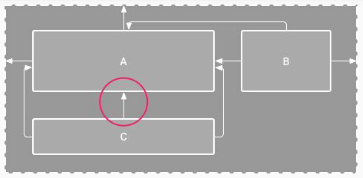
\includegraphics[width=0.5\textwidth]{foto1.png}
\end{center}
Come da raffigurazione è evidenziata la presenza di un vincolo tra l'entita A e l'entità C; è denominato \textbf{punto di ancoraggio}, in questo caso rappresentativo di un \textit{constraint} di tipologia \textit{top}.\vspace*{14pt}\\ 
\textit{ConstraintLayout} sono caratterizzati da una complessa e verbosa sintassi; proprio per questa ragione in Android Studio è predisposto un \textit{editor} in grado di posizionare manualmente vincoli tra \textit{Layout}, \textit{View} oppure, più generalmenete, elementi grafici, e di visualizzare una anticipazione della modellazione in atto.

\subsection*{RecyclerView}
Una \textbf{RecyclerView} è attuata per visualizzare in maniera efficiente grandi insiemi di dati. Pertanto fornendo i dati di riferimento e definendo la modalità in cui essi debbano apparire, la \textit{RecyclerView} dinamicamente crea gli elementi grafici e li dispone a video dove vi sia la necessità. \vspace*{14pt}\\
Pertanto, rende facile la visualizzazione di grandi moli di informazioni, da cui si evidenzia la presenza di molteplici layout dedicati ad ogni insieme di membri.\vspace*{14pt}\\
Tutto ciò che è stato descritto può essere attuato attraverso un esempio, in cui le \textit{ListView} acquisiscono la predominanza; meccanismo tramite il quale è possibile aggiungere, rimuovere e aggiornare il contenuto posto al loro interno durante runtime, senza che ogni volta sia completamente ridisegnata la \textit{ViewGroup}. A conoscenza di questo scopo sono implementati alcuni metodi specifici, come:
\begin{enumerate}
  \itemsep0em
  \renewcommand{\labelenumi}{-}
  \item \textbf{notifyDataSetChanged()}, ...
  \item \textbf{notifyItemInserted()}, ...
  \item \textbf{notifyItemUpdated()}, ...
  \item \textbf{notifyItemDeleted()}, ...
\end{enumerate}
Adeguandosi alle caratteristiche osservate, il caso di studio proposto pone come obiettivo da conseguire la creazione di una \textit{ListView} contenente elementi visivi \textit{TODO}, composti a loro volta da una \textit{TextView} e da una \textit{CheckBox}. I passi necessari per riuscire nell'intento sono cosi suddivisi:
\begin{enumerate}
  \itemsep0em
  \renewcommand{\labelenumi}{-}
  \item Definire il layout dell'elemento grafico, in questo caso dell'oggetto \textit{TODO}. In tale ambito una buona scelta implementativa prevede l'utilizzo di una \textit{CardView}, rappresentante un contenitore che mostra sequenzialmente i dati immessi al suo interno\\
  \begin{lstlisting}[language=XML, title=Definizione della CardView degli elementi TODO]
<androidx.cardview,.widget.CardView

</androidx.cardview.widget.CardView>
  \end{lstlisting}
  \item Definire la classe degli elementi \textit{TODO}. I \textit{TODOs} sono composti da un titolo testuale, incastonato all'interno di una \textit{TextView}, e da un valore booleano, definito per la \textit{CheckBox}\\
  \begin{lstlisting}[language=JAVA, title=Definizione della classe TODO]
data class Todo {
  var todoTitle: String,
  var done: Boolean = false
}
  \end{lstlisting}
  \item Definire la \textit{ViewHolder}. La \textit{ViewHolder} consiste in un \textit{contaneir} in grado di mantenere tutte le referenze alle proprie \textit{children view}, in modo tale che le stesse possano essere modificate durante \textit{runtime}\\
  \begin{lstlisting}[language=JAVA, title=Definizione della ViewHolder]
class TodoViewHolder(itemView: View): ViewHolder(itemView) {
  val tvTodoTitle: TextView = itemView.findViewById(R.id.todoTitle)
  val cbDone: CheckBox = itemView.findViewById(R.id.todoCheck)
}
  \end{lstlisting}
  \item Definire un \textit{Adapter}. L'\textit{Adapter} è una parte fondamentale per lo sviluppo e il funzionamento di una \textit{RecyclerView} poichè capace di acquisire in input un insieme di dati, in questo caso di studio si trattano di oggetti \textit{TODO}, e di generare per ogni \textit{Entry} elaborata una \textit{ViewHolder}, compiendo un'essenziale attività di \textit{override}
  \begin{lstlisting}[language=JAVA, title=Definizione dell'Adapter]
class TodoAdapter (private val todos: MutableList<Todo>): Adapter<TodoViewHolder>() {
  override fun onCreateViewHolder(parent: ViewGroup, viewType: int): TodoViewHolder (...)
  override fun onBindViewHolder(holder: TodoViewHolder, position: int): {...}
  override fun getItemCount(): int {...}
}
  \end{lstlisting}
  \item In questa breve sezione si commenta il funzionamento di ogni metodo che contraddistingue l'esempio di codice precedente, in cui: 
  \begin{itemize}
    \itemsep0em
    \renewcommand{\labelenumi}{-}
    \item \textbf{onCreateViewHolder()}, funzione invocata qualora un nuovo elemento debba essere inserito. Formulata in maniera tale che la \textit{ViewHolder} abbia al suo interno il layout corretto; tuttavia è ancora vuota, ossia devono essere associati i valori correnti all'oggetto TODO mantenuto al suo interno. La fase di \textit{bind} dell'elemento grafico e delle sue caratteristiche avviene solamente qualora dettata una posizone all'interno della \textit{RecyclerView}\\
    \begin{lstlisting}[language=JAVA, title=Creazione della ViewHolder]
override fun onCreateViewHolder(parent: ViewGroup, viewType: int): TodoViewHolder {
  return TodoViewHolder(
    Layoutinflater.from(parent.context).inflate(R.layout.todo_card, parent, false)
  )
}
    \end{lstlisting}
    \item \textbf{onBindViewHolder()}, metodo attuato nel momento in cui sia data una posizione al nuovo elemento \textit{TODO} all'interno della \textit{RecyclerView}; proprio in questo istante sono popolati i field dell'oggetto 
    \begin{lstlisting}[language=JAVA, title=Popolamento dell'elemento grafico]
override fun onBindViewHolder(holder: TodoViewHolder, position: int) {
  holder.apply {
    tvTodoTitle.text = todos[position].todoTitle
    cbDone.apply{
      isChecked = todos[position].done
      setOncheckedChangeListener(_, b -> todos[position].done = b)
    }
  }
}
    \end{lstlisting}
    \item \textbf{getItemCount()}, \textit{helper function} attuata per restituire il numero di elementi presenti all'interno della struttura dati
    \begin{lstlisting}[language=JAVA, title=Return degli elementi della lista di TODO]
override fun getItemCoun(): Int {
      return todos.size;
}
    \end{lstlisting}
  \end{itemize}
  \item Assegnare un \textit{LayoutManager} alla \textit{RecyclerView}. In questo modo è applicato uno "stile" visivo ai differenti elementi grafici  
  \begin{lstlisting}[language=JAVA, title=Assegnamento del layout ai nuovi oggetti grafici contenuti nela RecyclerView]
val recyclerTodo: RecyclerView = findViewById(R.id.recyclerTodo)
recyclerTodo.adapter = TodoAdapter(mutableListOf())
recyclerTodo.layoutManager = LinearLayoutManager(this)
  \end{lstlisting}
\end{enumerate} 
\end{document}